\section{Performance Assessment}

We pursue a quantitative understanding of the performance of our method by considering a sphere of radius $R$ and center $\bm{C}$.  We assign a material identifier $m$ to each voxel in the image to define our spherical image mask; for the voxel with center at $\bm{v}$, the material assignment is:
\begin{linenomath}\begin{align} 
	m &=  \begin{cases}
		1, & \text{if}\ d \left(\bm{v},\bm{C}\right) \le R \\
		0, & \text{otherwise},
	\end{cases}
\end{align}\end{linenomath}
where $d(\cdot,\cdot)$ is the Euclidean distance. The voxel grid has dimensions $256 \times 256 \times 256$.
%%%%%%%%%%%%%%%%%%%%%%%%%%%%%%%%%%%%%%%%%%%%%%%
%%%%%%%%%%%%%%%%%%%%%%%%%%%%%%%%%%%%%%%%%%%%%%%
\subsection{Error Measures}
\label{Error Measures}

Two error metrics are defined: a {\em shape error} and a {\em volume error}. These metrics characterize the departure of the b-rep from an exact sphere. There are two sources of error~\cite{young_2008}: 1) error due to approximating the sphere with a binary image mask, or the {\em image-based error}; and 2) error due to reconstructing the binary image mask with a facetized b-rep. The latter dictates a method's ability to {\em converge to geometry}. The image mask defined above does not, of course, yield perfect image-based accuracy. In general, the object being scanned and segmented may not be well-defined or characterized, and as such, the image-based error is difficult to quantify. For this reason we select a sphere for quantitative comparison so that we have an analytical representation of what the true result should be. In this way we need not make assumptions about the image-based error, and can directly compare the facetized b-rep to the original intended object before it is even digitized into a raw image.

The shape error measures the surface-normal deviation of our algorithm's end-result b-rep from the exact sphere. The measure is constructed first by projecting each facet of the b-rep onto the exact sphere. The normal of each facet is compared to the normal of the exact sphere at the centroid of the projected facet by computing the magnitude of their cross product. An area-weighted sum is then taken over the b-rep, and finally the sum is normalized by the surface area of the b-rep. The error measure therefore lies in the range $\left [0,1\right]$. The shape error $e_s$ formula is:
\begin{equation} 
	e_s = \frac{ \sum \limits_{f\in\mathcal{F}} A_f \lVert {\bf n}_f \times {\bf n}_s \rVert}{\sum \limits_{f\in\mathcal{F}} A_f},
\end{equation}
where $A_f$ is the area and ${\bm n}_f$ is the unit normal of facet $f$, $\mathcal{F}$ is the set of all b-rep facets, and ${\bm n}_s$ is the normal of the exact sphere at the centroid of the projected facet onto the sphere.

The volume error measures the unsigned volume enclosed between the b-rep and the exact sphere. We calculate this measure via a sum of integrals over the projections $\gamma_f$ of each facet onto the exact sphere: 
\begin{equation}
\label{vol err}
	e_v = \frac{1}{4\pi R^2} \Big[\sum \limits_{f \in \mathcal{F}} \int \limits_{\gamma_f} (r - R)^2 d\alpha \Big]^{1/2} .
\end{equation}
Here, $r = \lVert {\bm x} \rVert$ is the distance from the sphere center to points on the planar facet associated with the projection $\gamma_f$, and $R$ is the radius of the exact sphere.  The indicated integrals are performed numerically on the projected facets. Six quadrature points were found to provide sufficient accuracy. The volume error is made dimensionless by normalizing by the surface area of the exact sphere.
%%%%%%%%%%%%%%%%%%%%%%%%%%%%%%%%%%%%%%%%%%%%%%%
%%%%%%%%%%%%%%%%%%%%%%%%%%%%%%%%%%%%%%%%%%%%%%%
\subsection{The Unpolluted Sphere}
\label{The Unpolluted Sphere}

The shape and volume errors were computed for the proposed method and for the three comparison approaches, for a perfect sphere embedded in a fixed $256 \times 256 \times 256$ array of voxels.  In the comparisons presented below, three independent parameters were varied:  1) b-rep resolution, 2) sphere radius, and 3) sphere-center location relative to the voxel grid. The purpose of these comparisons for clean input masks is to show that the proposed method performs comparably to other options, rather than specifically pointing to the superiority of one method over the other.

\figref{graph1} shows the shape and volume errors of the four methods as the b-rep resolution is varied for a spherical mask centered in the image with radius $R = 80$ voxels. See \figref{demos1} for a visual comparison of the image mask with representative b-reps from the proposed method and the other approaches. Default parameters were used in Simpleware for b-reps with $n \ge 2587$ vertices. For resolutions coarser than that, the ``target maximum error" was increased to allow results with $n < 2587$. When comparing the shape error of the different approaches, the proposed method performs competitively for coarse meshes ($n < 2500$), while it performs measurably better -- up to $40\%$ improvement -- for finer b-reps ($n > 5000$). Note that the shape error for marching cubes grows for higher b-rep resolutions due to aliasing -- when more points are used, the decimation step suppresses marching cubes' stair-step effect less strongly. Although the proposed method is subject to aliasing as well, this result suggests that the effect is significantly less than as is seen with marching cubes.  For the volume error, the proposed method performs up to $70\%$ better for b-reps with resolutions of $n < 5000$ vertices, and converges to a comparably small, but nonzero value as that of the other methods.  Note however that the volume errors are quite small for {\em all} methods tested.
\begin{figure}[b!]
\centering
\subfigure[]{%
	\includegraphics[scale=0.28]{media/7-performance/graph-resolution-shape.pdf}}
\subfigure[]{%
	\includegraphics[scale=0.28]{media/7-performance/graph-resolution-volume.pdf}}
%	
\caption{Comparison of (a) shape error and (b) volume error of the proposed method to those of the three comparison methods as the b-rep resolution is varied.}
\label{fig:graph1}
\end{figure}
\begin{figure}[t!]
	\centering
	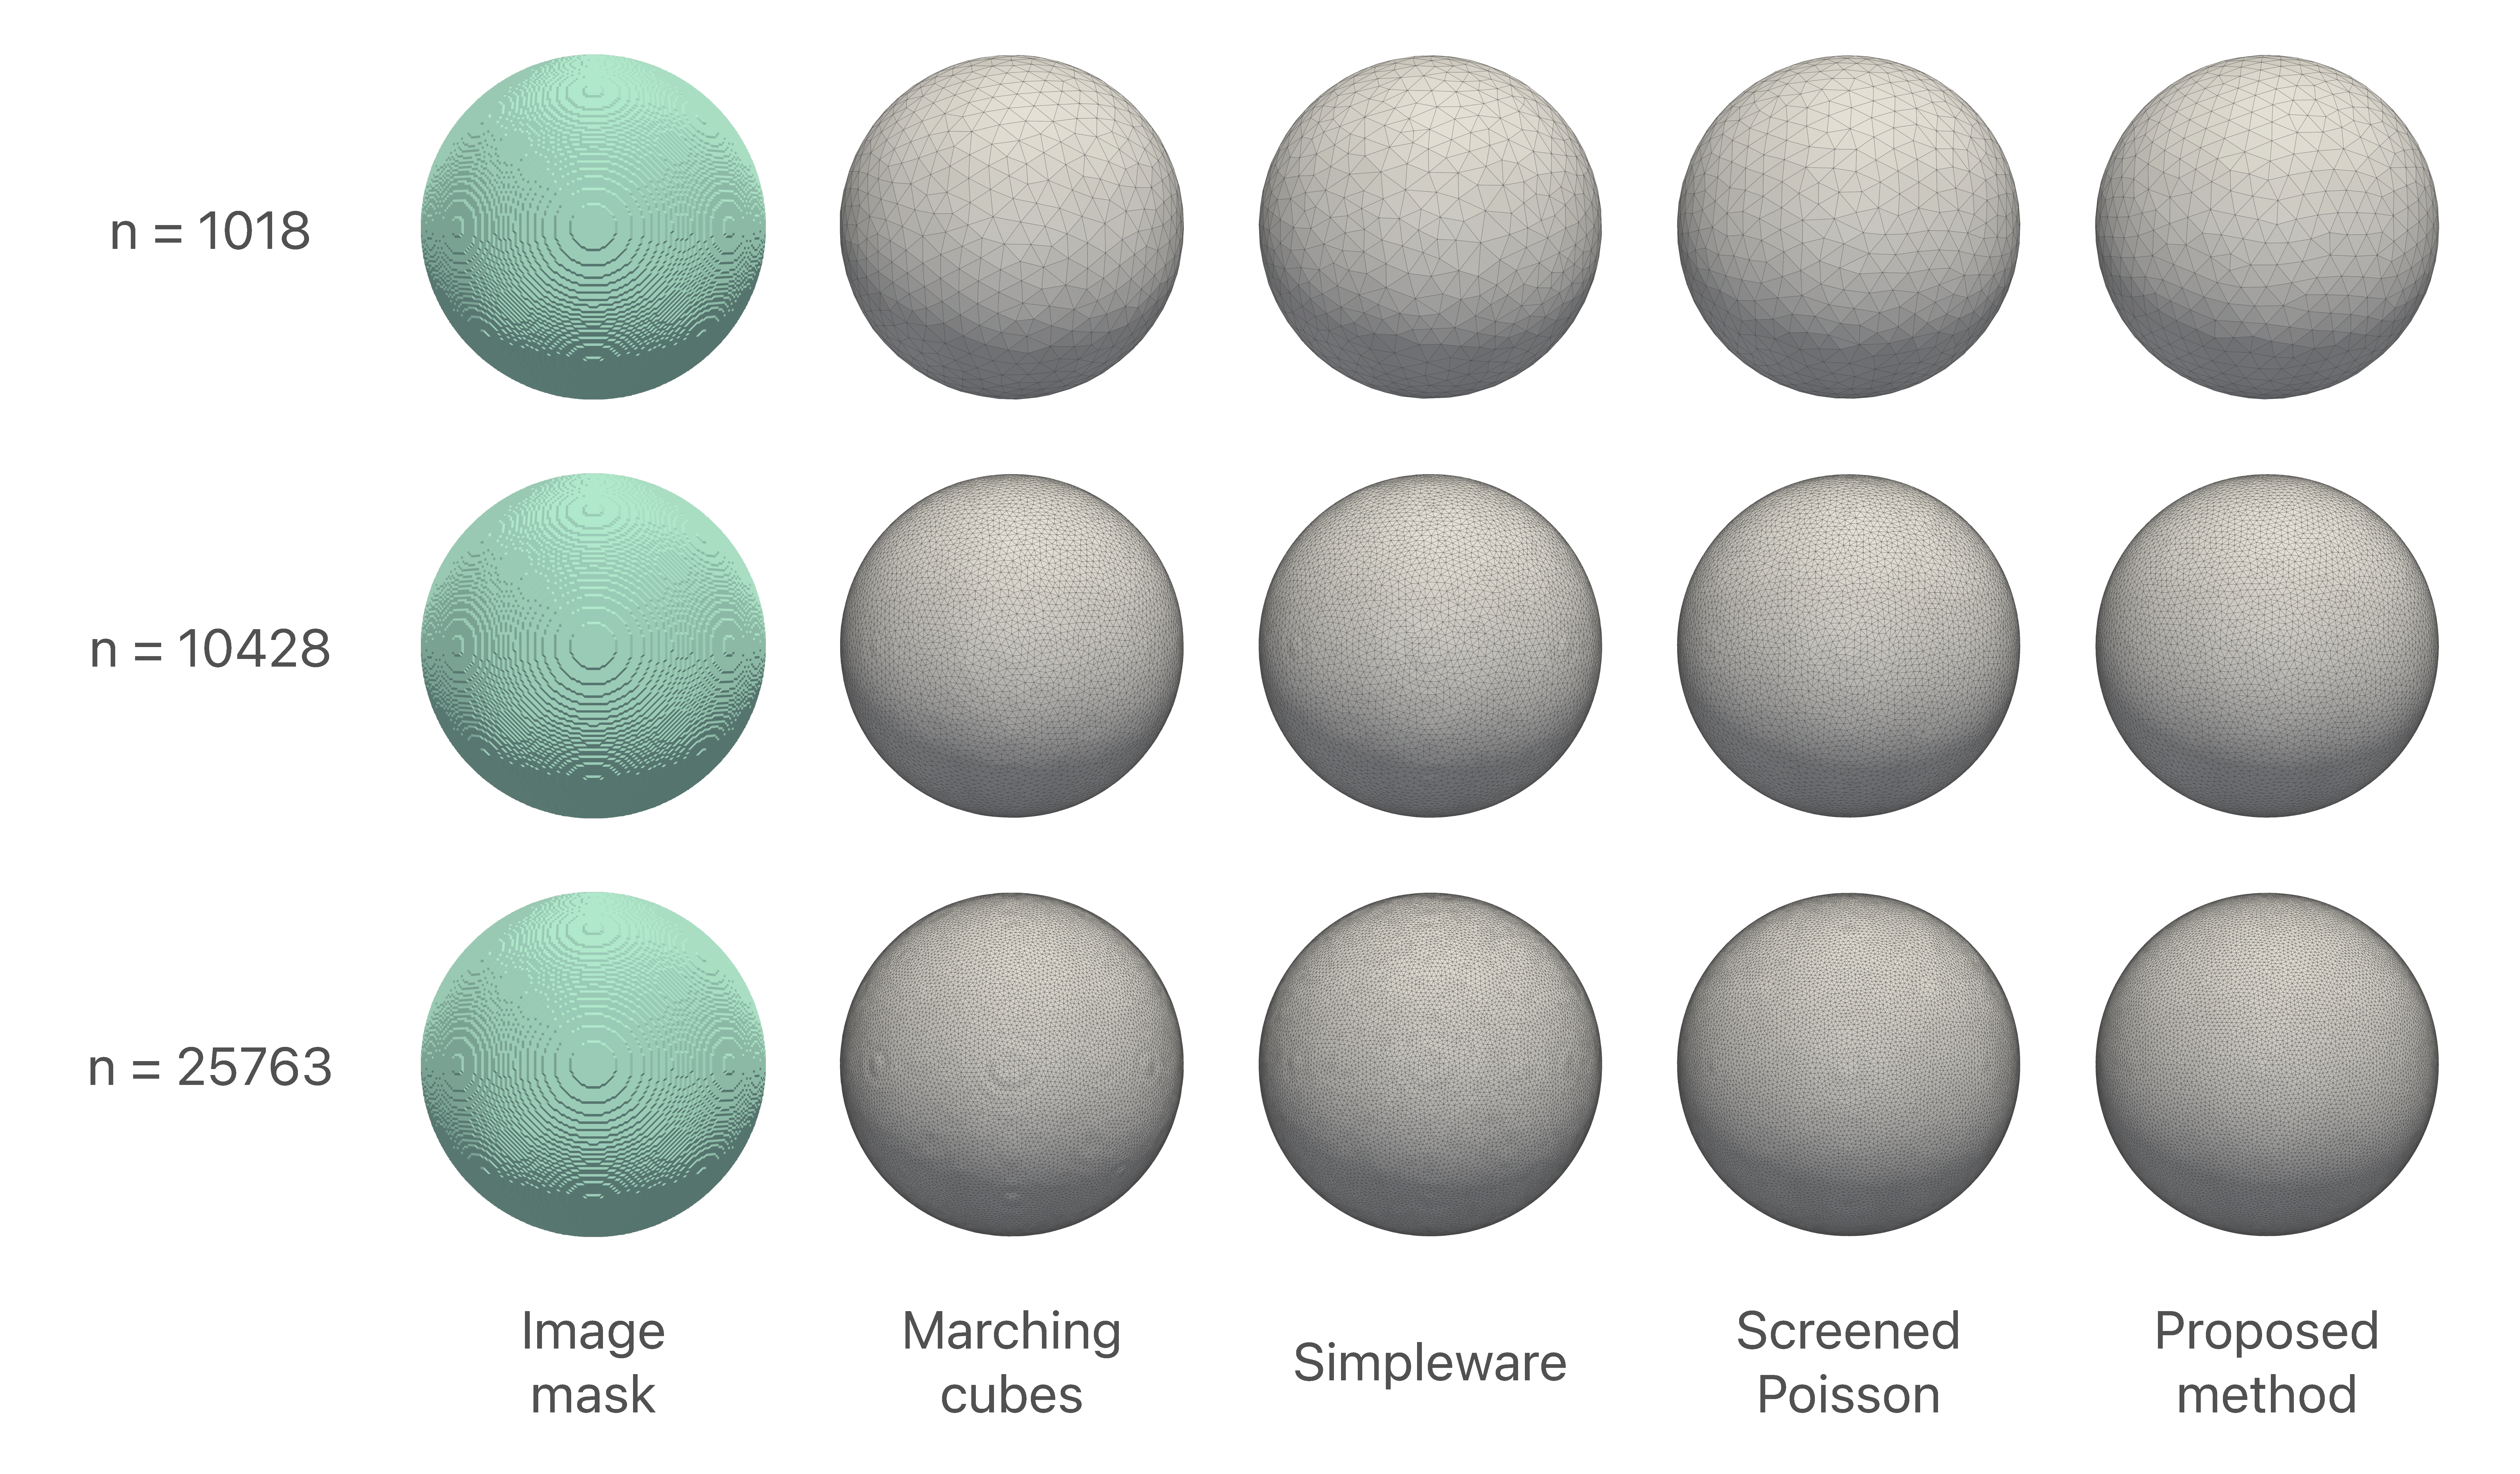
\includegraphics[scale=0.10]{media/7-performance/spheres-resolution.pdf}
	\caption{Comparison of proposed method with different approaches for selected b-rep resolutions.}
	\label{fig:demos1}
\end{figure}

\figref{graph2} shows the error metrics when the radius of the spherical mask is varied from 40 to 120 voxels, while keeping the sphere centered in the image and the b-rep resolution fixed at $n = 10428$ vertices. See \figref{demos2} for representative examples of the image mask and resulting b-reps for the different methods. The sphere radius represents an inverse measure of the curvature of the image mask relative to the voxel resolution; larger radii correspond to smoother surfaces. Both the shape and volume errors of the proposed method converge at least as quickly as the other methods, with the exception of the shape error for marching cubes, which has a noticeably larger error for smaller radii. The proposed method's shape error is the lowest of all methods tested over the entire range of sphere radii considered.  The volume error is very small for all methods over the range of sphere radii considered, but Simpleware and marching cubes exhibit some advantage over the proposed method and screened Poisson, particularly for small spheres.

\begin{figure}[b!]
	\centering
	\subfigure[]{%
		\includegraphics[scale=0.28]{media/7-performance/graph-size-shape.pdf}}
	\subfigure[]{%
		\includegraphics[scale=0.28]{media/7-performance/graph-size-volume.pdf}}
	%	
	\caption{Comparison of (a) shape error and (b) volume error of proposed method with different approaches as the sphere radius is varied.}
	\label{fig:graph2}
\end{figure}
\begin{figure}[t!]
	\centering
	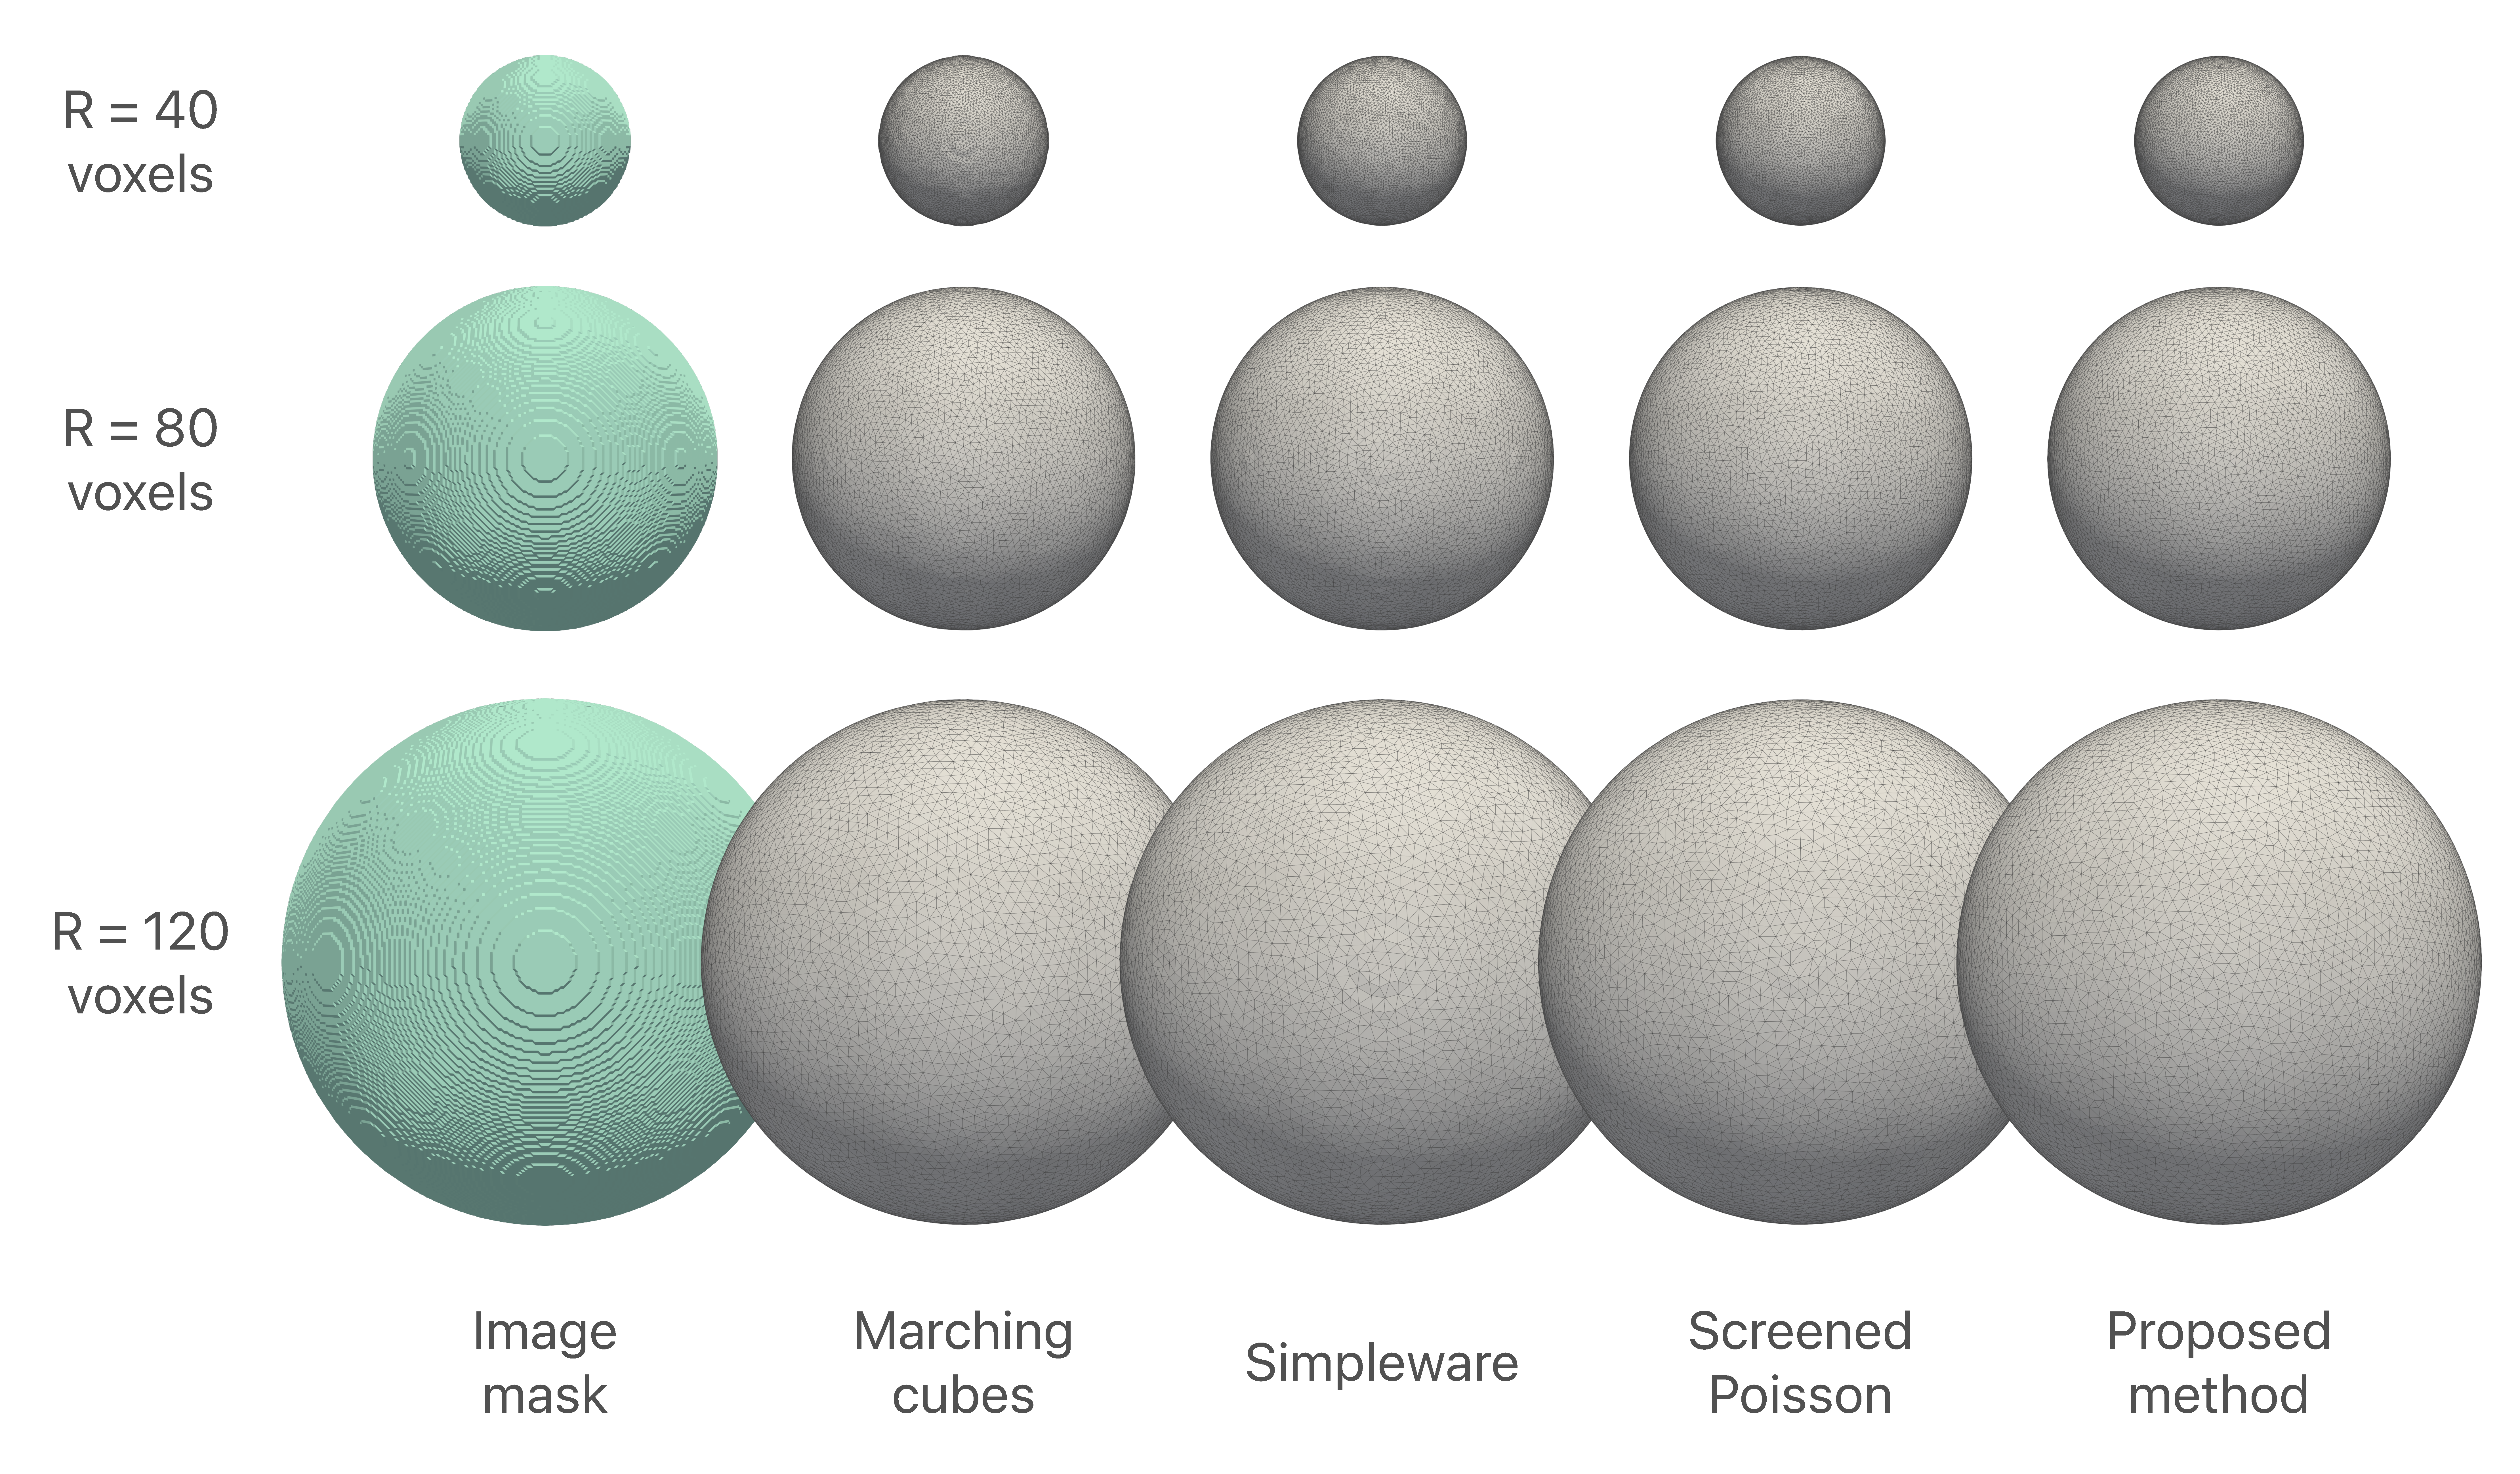
\includegraphics[scale=0.10]{media/7-performance/spheres-size.pdf}
	\caption{Comparison of proposed method with different approaches for selected sphere radii.}
	\label{fig:demos2}
\end{figure}

The methods are also compared for a sphere of $R = 80$ voxels that is translated along the direction $\bm{i}  + 2\bm{j} + 3\bm{k}$, while keeping the resolution fixed at $n = 10428$ vertices.  All methods show very low sensitivity to the translation of the object within the image, as shown in \figref{graph3}. The proposed method exhibits a relative standard deviation (RSD) that is smallest among the group in shape error ($1.1\%$), and highest in volume error ($2.1\%$). For reference, the RSDs of marching cubes, Simpleware, and screened Poisson surface reconstruction were $1.4\%$, $2.4\%$, and $1.9\%$ for shape error, and $1.3\%$, $1.7\%$, and $1.6\%$ for volume error.

\begin{figure}[b!]
	\centering
	\subfigure[]{%
		\includegraphics[scale=0.28]{media/7-performance/graph-center-shape.pdf}}
	\subfigure[]{%
		\includegraphics[scale=0.28]{media/7-performance/graph-center-volume.pdf}}
	%	
	\caption{Comparison of (a) shape error and (b) volume error for the four methods as the sphere center is translated.}
	\label{fig:graph3}
\end{figure}
%%%%%%%%%%%%%%%%%%%%%%%%%%%%%%%%%%%%%%%%%%%%%%%
%%%%%%%%%%%%%%%%%%%%%%%%%%%%%%%%%%%%%%%%%%%%%%%
\subsection{{The Polluted Sphere}}
\label{The Polluted Sphere}

As a final point of quantitative comparison, the proposed method is compared to the other approaches as synthetic noise is introduced into the image mask. Specifically, voxel values are randomly flipped near the boundary of the sphere. This was done for a sphere with $R = 80$ voxels, and keeping the b-rep resolution as close to 10428 vertices as possible. Because the introduction of noise did create artifacts for some of the methods that produced higher resolutions in unpredictable ways, we were unable to strictly adhere to this value. It was, however, verified that the b-rep resolution negligibly affected the results when studying the introduction of noise. \figref{graph4} shows shape and volume errors for the four methods as the percentage of randomly-flipped voxels near the boundary, or the {\em noise ratio}, is increased from $0\%$ to $20\%$. See \figref{demos4} for representative images.  For the proposed method, the shape and volume errors remain low, even for large values of the noise ratio. This tends to confirm the robustness of the proposed method in the presence of low-quality image-mask inputs. 
\begin{figure}[t!]
	\centering
	\subfigure[]{%
		\includegraphics[scale=0.28]{media/7-performance/graph-noise-shape.pdf}}
	\subfigure[]{%
		\includegraphics[scale=0.28]{media/7-performance/graph-noise-volume.pdf}}
	%	
	\caption{Comparison of (a) shape error and (b) volume error of the four approaches as a function of noise ratio.}
	\label{fig:graph4}
\end{figure}
\begin{figure}[b!]
	\centering
	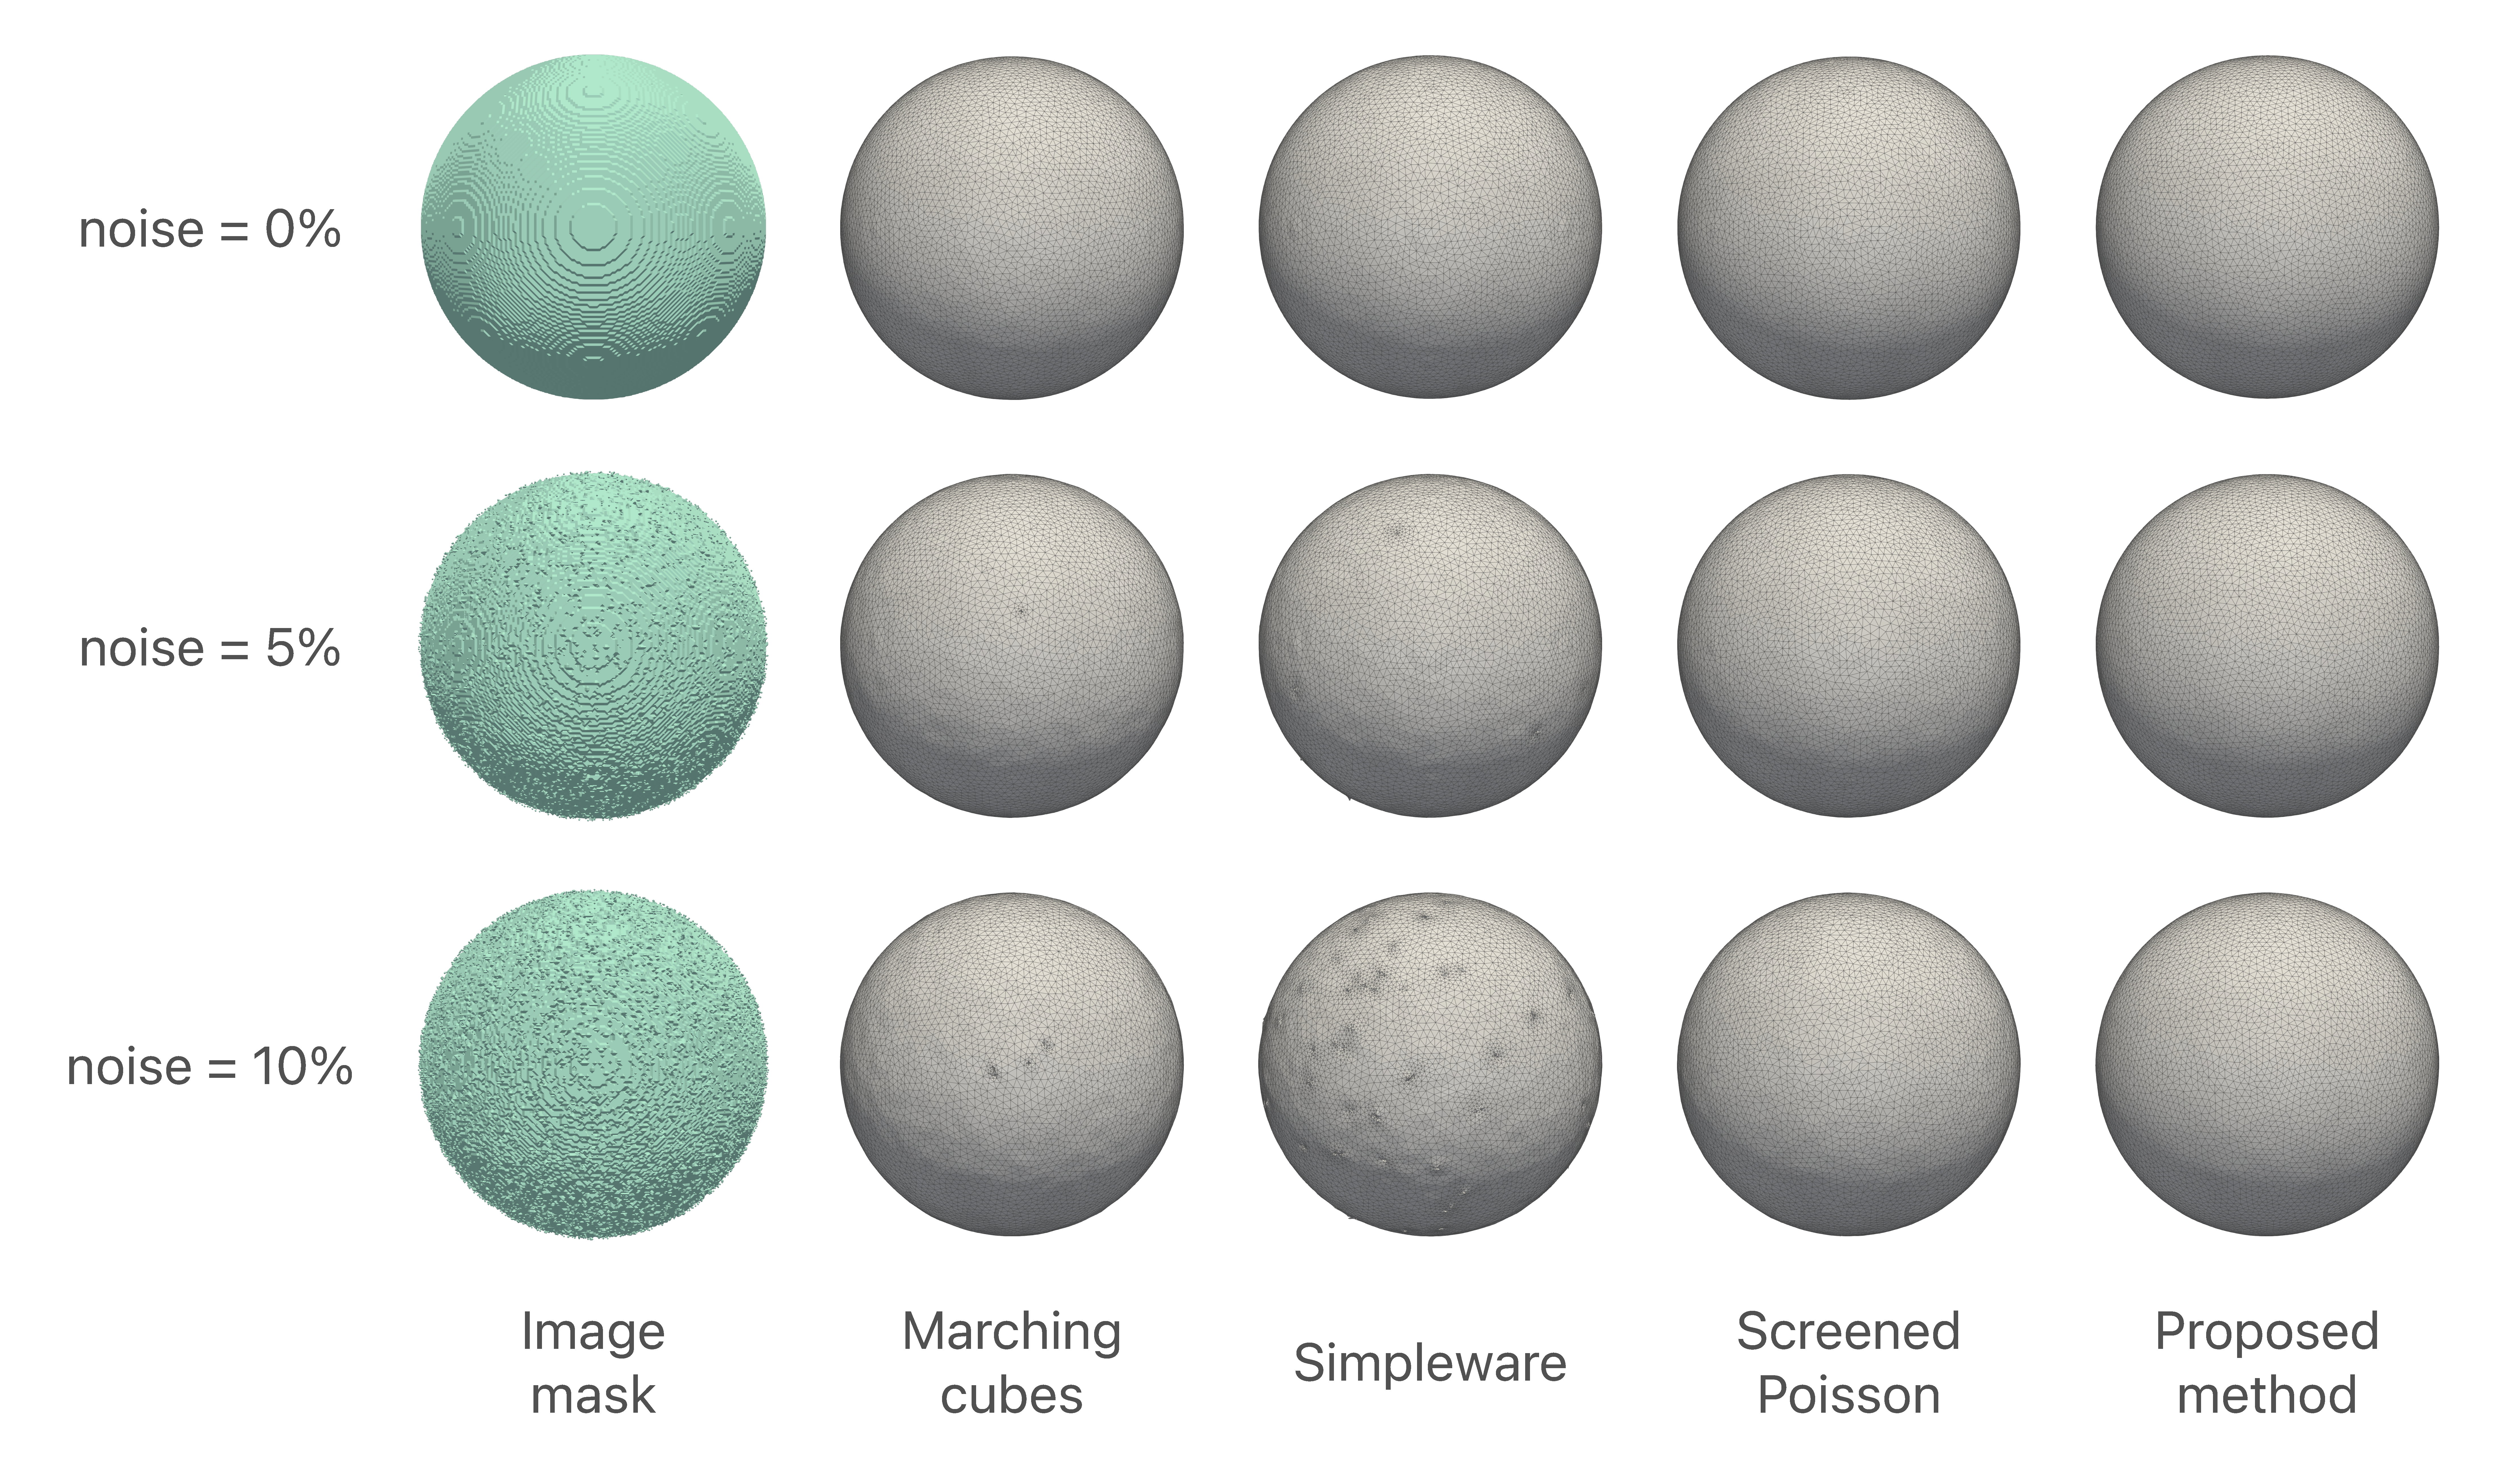
\includegraphics[scale=0.10]{media/7-performance/spheres-noise.pdf}
	\caption{{Comparison of proposed method with different approaches for selected mask noise.}}
	\label{fig:demos4}
\end{figure}

%%%%%%%%%%%%%%%%%%%%%%%%%%%%%%%%%%%%%%%%%%%%%%%
%%%%%%%%%%%%%%%%%%%%%%%%%%%%%%%%%%%%%%%%%%%%%%%
\subsection{Complex Surfaces}
\label{Complex Surfaces}

Lastly, we present several qualitative comparisons based on real image masks generated from MRI and CT.  All images were segmented using \textit{Seg3D} \cite{Seg3D}.  B-rep resolutions were matched in all cases, to make for a fair comparison. All examples completed for the proposed method on a 16 GB RAM laptop in less than 5 minutes. See \figref{example-meshes} for comparisons of the image masks and resulting b-reps. Visual inspection suggests that the proposed method qualitatively performs comparably to the {other approaches} in all cases, performing slightly better for smooth surfaces and not quite as well for regions with high curvature. In this connection, we mention that the proposed method readily accommodates an enhancement that admits sharp edges and vertices (or corners), making the method particularly suitable for industrial applications involving manufactured objects.  Work on this enhancement is in progress.  The suite of examples presented here nonetheless show a robustness and quality that illustrate the proposed method as a viable approach as it stands.

\begin{figure}[h!]
	\centering
	 \includegraphics[scale=0.145]{media/7-performance/realExamples072022.pdf}
	\caption{{Comparison of proposed method with different approaches for various input image masks generated from MRI and CT scans. Note the proposed method's robustness to noisy inputs for the brain (second), distal femur (third), and equine proximal sesamoid (bottom). Sources: heart~\cite{cvgg}, brain~\cite{marcus_2007}, distal femur~\cite{epperson_2013}, pelvis~\cite{clark_2013}, L5 lumbar~\cite{yao_2016}, and equine proximal sesamoid~\cite{shaffer2021}}}
	\label{fig:example-meshes}
\end{figure}

Of note, too, is the proposed method's performance for noisy image masks, namely the brain, distal femur, and equine proximal sesamoid. The brain and distal femur masks were generated from MRI scans, and the proximal sesamoid from CT, showing that noise may come from either scanning modality.  For these cases, the b-reps produced by marching cubes and Simpleware exhibit artifacts due to the noise in the input image mask.  Both the screened-Poisson approach and the proposed method show more resilience to the noise.  In general, the proposed method comparably to the other approaches of interest, demonstrating the ability of our contributions in point cloud generation and Voronoi-based surface reconstruction in reliably generating b-reps from real-world image masks.

It is important to emphasize again that image masks were produced in Seg3D, that is, outside of Simpleware. As a result, image masks were binary, and did not include any partial volume information that may have been stored in Simpleware based on the background image. The intent of this was to be able to compare all results based on the same input image masks. Granted, Simpleware would have performed better had the original raw images been segmented within its own software ecosystem, so that it could take advantage of its ability to utilize partial volume information. That said, in practice it is not unrealistic to receive a segmented image that was produced from a different software, and without access to the raw background image altogether. It is also important to note that, Simpleware does have tools to address noisy image masks. In reality, additional smoothing and filtering would have been applied prior to meshing. For both of these reasons, the intention is not to show that marching cubes and Simpleware cannot produce high quality b-reps from those particular examples, but rather, that additional steps would have needed to be taken, whereas the proposed method showed the ability to produce high-quality results even in the presence of that noise.  Again this is an unrealistic assumption to make, that one might want to produce b-reps from noisy image masks with as few cleanup steps as possible. This is especially true as the industry moves toward automatically segmenting large sets of image data via machine learning techniques, in which it may be untenable to hand pick the image segmentations that require additional cleaning, or globally applying additional cleaning steps that may not be necessary for the majority of segmentations. All that said, we repeat that the intention is not to show the superiority of our method, but rather only that it performs comparably and competitively with other respected approaches.

The ``marching cubes'' approach applies the same decimation and smoothing as the proposed method following conventional marching cubes, for fair comparison. The ``Screened Poisson'' approach applies Screened Poisson surface reconstruction on oriented point clouds generated from the scheme described in the proposed method.